
\begin{frame}
\frametitle{Market Entry Game}
\begin{itemize}
\item Consider this variation on the Entry Game, in which the Entrant is not as efficient as the Incumbent:
\end{itemize}
\begin{figure}
	\begin{minipage}{0.49\linewidth}
		\centering
		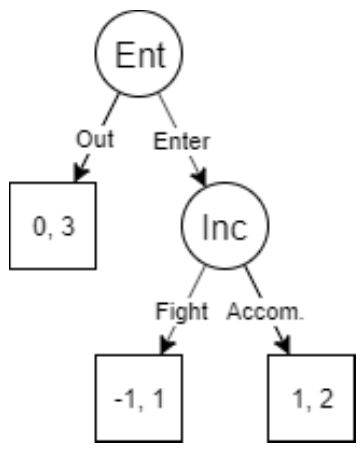
\includegraphics[width=0.55\textwidth]{figures/08InferiorEntrant.png}
	\end{minipage}
	\begin{minipage}{0.49\linewidth}
		\begin{tabular}{cc|c|c|}
			& \multicolumn{1}{c}{} & \multicolumn{2}{c}{Incumbent}\\
			& \multicolumn{1}{c}{} & \multicolumn{1}{c}{$Fight$}  & \multicolumn{1}{c}{$Accom.$} \\\cline{3-4}
			\multirow{2}*{Entrant}  & $Enter$ & -1, 1 & 1, 2 \\\cline{3-4}
			& $Out$ & 0, 3 & 0, 3 \\\cline{3-4}
		\end{tabular}
	\end{minipage}
\end{figure}
\begin{itemize}
\item Note that this game has two NEs: (Enter, Accommodate) and (Out, Fight). 
\item Does it really make sense for the Incumbent to ever Fight?
\end{itemize}
\end{frame}

\begin{frame}
\frametitle{Refining Nash Equilibrium}
\begin{itemize}
\item The more you think about it, the less sense this Nash equilibrium makes.
\item The only reason why the Entrant would choose to stay Out is if they really, truly believe that if they Entered, the Incumbent would Fight.
\item \dots but it's hard to justify that belief when Fighting is costly for the Incumbent.
\begin{itemize}
\item The Incumbent would have to somehow convince the Entrant that they really would Fight them, perhaps by making a \alert{credible threat}.
\item We will talk more about this kind of \alert{strategic move} later in the course.
\end{itemize}
\item We often don't want this kind of Nash Equilibrium. To rule it out, we have the concept of \alert{subgame perfection}.
\end{itemize}
\end{frame}

\begin{frame}
\frametitle{Subgames}
\begin{itemize}
\item A \alert{subgame} is a subset of an extensive-form game which, itself, is a complete game.
\item In the context of a game tree, a subgame is a \textbf{single node}, and all of the branches and nodes descending from it, such that it forms a complete game.
\end{itemize}
\end{frame}

\begin{frame}
\frametitle{Examples of Subgames}
\begin{itemize}
\item Each of these green boxes contains a subgame.
\end{itemize}
\begin{figure}
\centering
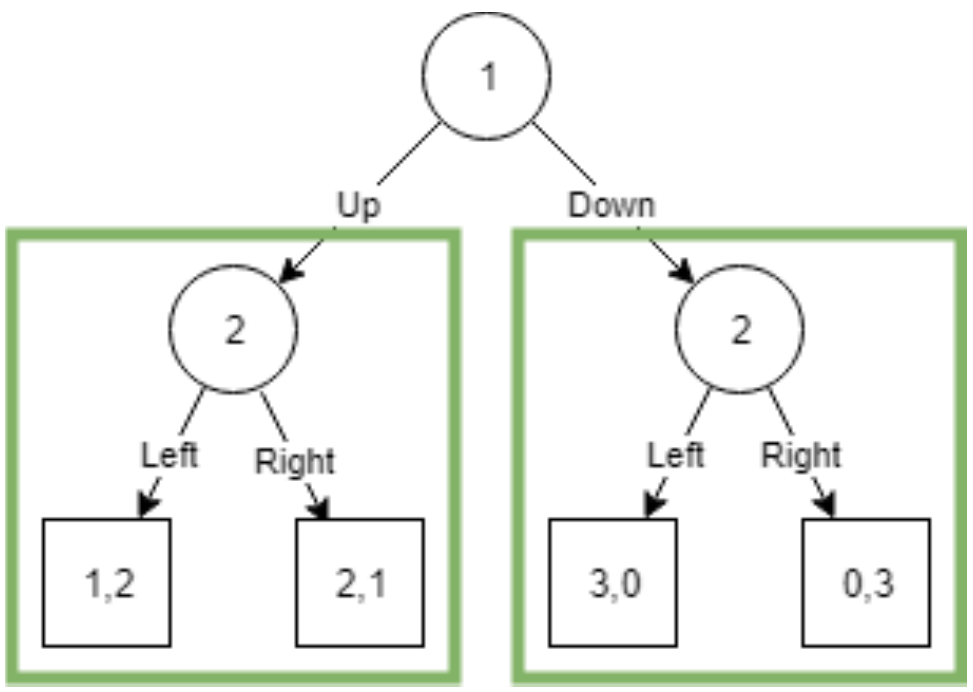
\includegraphics[width=0.75\textwidth]{figures/06SubgameExample01.png}
\end{figure}
\end{frame}

\begin{frame}
\frametitle{Examples of Subgames}
\begin{itemize}
\item Each of these green boxes contains a subgame.
\begin{itemize}
\item The smaller boxes are \alert{trivial subgames}, because they don't contain any meaningful choices.
\end{itemize}
\end{itemize}
\begin{figure}
\centering
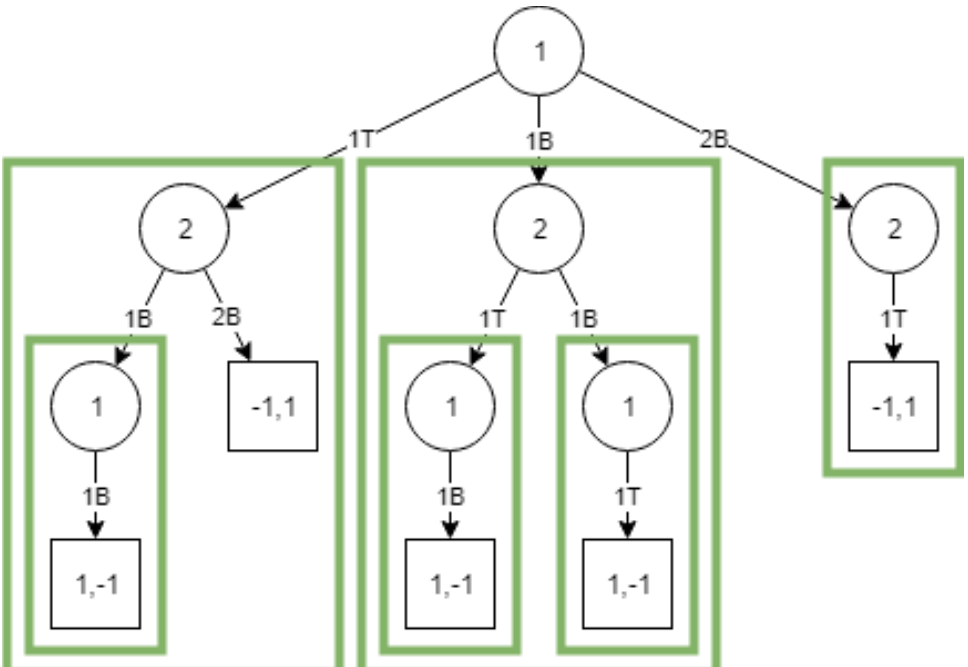
\includegraphics[width=0.75\textwidth]{figures/06SubgameExample02.png}
\end{figure}
\end{frame}

\begin{frame}
\frametitle{Examples of Subgames}
\begin{itemize}
\item A game is, technically, a subgame of itself, but it is an \alert{improper subgame}. (Any subgames other than the entire game are \alert{proper subgames}.)
\end{itemize}
\begin{figure}
\centering
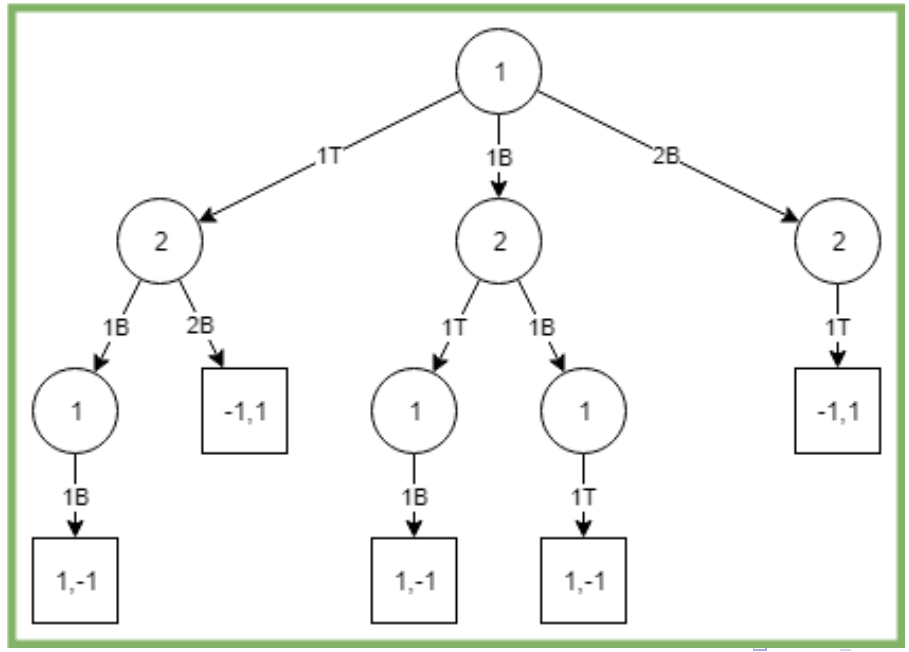
\includegraphics[width=0.7\textwidth]{figures/06SubgameExample03.png}
\end{figure}
\end{frame}

\begin{frame}
\frametitle{Subgame Perfection}
\begin{itemize}
\item So why do we care about subgames?
\item Because of a refinement of Nash equilibrium, called \alert{subgame-perfect Nash equilibrium}, that does not produce the questionable equilibria we saw earlier.
\item All subgame-perfect Nash equilibria are, obviously, regular Nash equilibria.
\item A subgame-perfect Nash equilibrium also has to produce a Nash equilibrium \textbf{in every subgame}.
\end{itemize}
\end{frame}

\begin{frame}
\frametitle{SPNE in the Entry Game}
\begin{itemize}
\item There is only a single proper subgame in the Entry Game.
\item A SPNE of this game must have a NE in that subgame.
\item The only NE of the subgame is for the Incumbent to Accommodate.
\end{itemize}
\begin{figure}
\centering
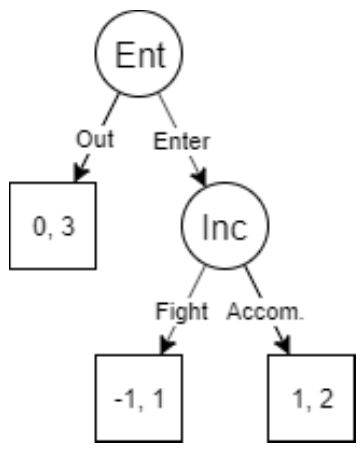
\includegraphics[width=.5\textwidth]{figures/08InferiorEntrant.png}
\end{figure}
\end{frame}

\begin{frame}
\frametitle{SPNE in the Entry Game}
\begin{itemize}
\item Given that the Incumbent Accommodates, the Entrant now faces a choice between staying Out, or Entering and being Accommodated.
\item The Entrant's best response is to Enter, and the SPNE is (Enter, Accommodate)
\end{itemize}
\begin{figure}
\centering
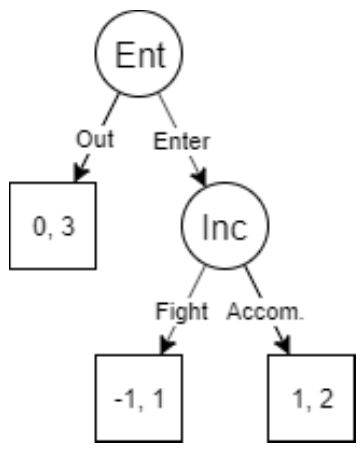
\includegraphics[width=.4\textwidth]{figures/08InferiorEntrant.png}
\end{figure}
\end{frame}

\begin{frame}
\frametitle{Rationality and Subgame Perfection}
\begin{itemize}
	\item To justify looking for SPNEs instead of NEs, we must make the assumption of \alert{commonly known sequential rationality}. There are two parts to this assumption:
	\begin{itemize}
		\item Players are aware that other players are sequentially rational.
		\item Knowing that other players are sequentially rational, each player can predict the others' rational behavior and will use this to choose an action which provides the largest possible payoff \textbf{at each node where they have a choice of actions}.
	\end{itemize}
	\item One way of thinking about this is that sequentially rational players choose their strategy ``on the fly," one move at a time, instead of all at once at the beginning of the game.
\end{itemize}
\end{frame}

\begin{frame}
\frametitle{Finding SPNEs: Backward Induction}
\begin{itemize}
\item The method for finding SPNEs is straightforward---we've already been using it without spelling it out formally.
	\begin{enumerate}
	\item Find all the decision nodes in the \textbf{lowest row} of decision nodes. (This assumes that the game tree is neat and orderly---which it will be if I'm giving you the game tree.)
	\item Find the optimal choice for players to make at each of these nodes, and mark the corresponding branch (or erase/cross out all the other branches).
	\item If you just solved the game's initial node, you're done! 
	\item Otherwise, identify all of the decision nodes in the \textbf{next row up} and return to step 2.
	\end{enumerate}
	\item At each step, remember to take into account the optimal moves that you've already found lower in the tree.
\end{itemize}
\end{frame}
